\chapter{Introduction}
\label{sec:intro} % Always give a unique label
\section{Motivation}
Many interventional procedures rely on needle insertion, including biopsy and brachytherapy\cite{bomers_mri-guided_2012}. Accurate needle placement is a critical factor in the success of these procedures\cite{nath_dosimetric_2000, youk_missed_2007}. Deflection of the needle tip during insertion and variation in the mechanical properties of tissue can cause the needle to deviate from its expected trajectory and miss the target. This can be mitigated by using an alignment structure to aim the needle at the target and verifying that the correct position has been reached in post-operative imaging\cite{tokuda_-bore_2012}. Even with preoperative image-based planning and careful alignment with the target, several insertions may be required to attain the desired needle placement\cite{onik_ct-guided_1988}. 

Live intra-operative imaging of the needle throughout insertion reduces error caused by needle deflection by allowing the surgeon to see if the needle is deviating from its trajectory and take corrective action. Ultrasound (US) and Magnetic Resonance Imaging (MRI) are preferred imaging modalities. While US is portable and hand-steerable, MRI offers superior resolution of soft tissues compared to both US and CT\cite{weiss_mr-guided_2008}. Manually-controlled image-guided needle insertion is still a challenging task. Under MRI guidance the confined space of the scanner bore, illustrated in Figure \ref{fig:mri_intraoperative}, limits the surgeon's visibility and range of motion\cite{damico_transperineal_2000, menard_mri_nodate}.

\begin{figure}[h]
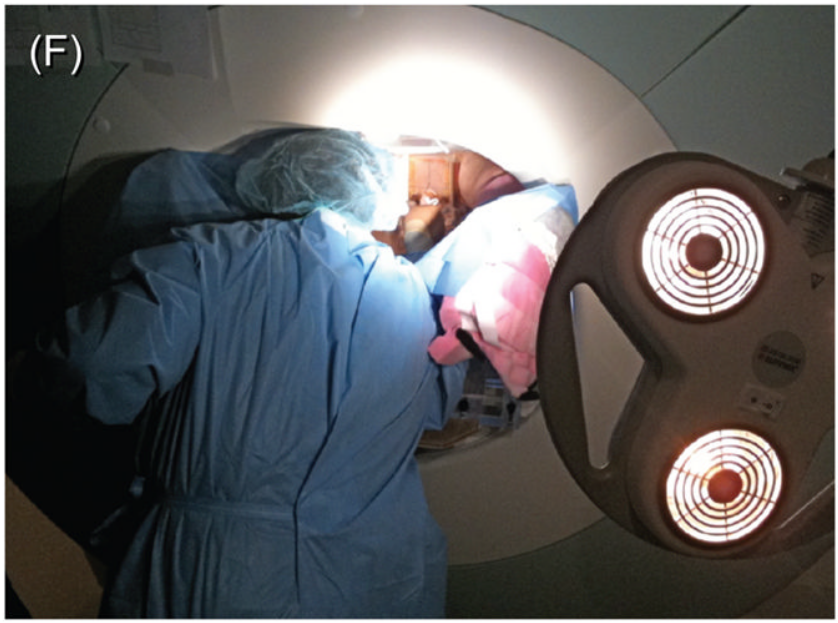
\includegraphics[width=1.0\textwidth]{Fig/chap1/tokuda_action_shot.png}
\caption{A manual MRI-guided biopsy in progress (from Tokuda, 2012 \cite{tokuda_-bore_2012}).}
\label{fig:mri_intraoperative}
\end{figure}

Robotically-controlled needle insertion solves some of the challenges of live intraoperative MRI imaging by reducing the clinician's workload and moving them out of the scanner bore. (CITE!)

Using live imaging, an insertion robot can correct for unmodeled tip deflection and keep the needle on its expected trajectory, improving the success rates of biopsies and other needle-based interventions. (CITE!)

Several collaborative needle insertion robots have been demonstrated. These allow the surgeon to control the rate of needle insertion while the robot controls the orientation of the needle. (CITE!)

Previous work has shown that closed-loop control of MRI\cite{patel_closed-loop_2015} and US\cite{vrooijink_needle_2014} coupled with image processing techniques for needle localization can track a needle tip during insertion with a useful degree of accuracy.

\section{Problem Formulation}
\label{sec:problem_formulation}
A key requirement in closed-loop image-guided needle insertion is the accurate measurement of the 6-degree-of-freedom pose of the needle tip using data from the imaging system. Accurate tip localization is required for the needle controller to determine the correct control input which minimizes the error between the current needle tip pose and the desired trajectory. Searching for the needle in each image on an individual basis introduces errors due to imaging artifacts, noise, and structures near the needle, contributing to reduced tip localization accuracy. A needle model that combines data from real-time imaging with the kinematics of the insertion platform and the mechanical properties of the needle would allow accurate estimation of the pose of the needle tip while requiring comparatively few observations of the needle position.

% - TODO: (Fischer) Why is accurate localization important?

\section{Thesis Contributions}

\subsection{Needle Modeling by Minimization of Bending Energy}
This thesis presents an approach to needle modeling that uses the mechanical bending properties of the needle, the pose of the needle base, and a set of observed needle positions along the needle shaft to find a configuration of the needle that minimizes its bending energy while meeting the observed constraints. In this model is represented by a three-dimensional parametric polynomial curve. 

\subsection{Imaging-Agnostic Needle Tip Localization Algorithm}
The needle model provides continuous needle pose estimates along its shaft, which can be used to plan imaging to observe the needle position after motion. The expected position of the needle informs the search for the actual position of the needle in received images, which reduces localization error caused by noise and other shapes near the needle. Since the needle model is updated using a set of positions along the needle shaft instead of the position of the needle tip, updates can be performed using imaging in planes transverse to the needle rather than imaging in the coronal and sagittal planes. This mitigates the risk of loss of needle tracking during insertion.

\subsection{MRI Data Collection}
MRI scans were collected depicting a biopsy needle being inserted into a gelatin tissue phantom. An alignment structure restricted the pose of the needle base during insertion, allowing each scan at a regular insertion interval to be associated with a needle pose.

\subsection{Slicer Module}
An extension for 3D Slicer, an open-source medical imaging program\cite{_3d_, fedorov_3d_2012}, was created to evaluate the needle model when applied to the MRI dataset. The user interacts with the needle model through the Needle Tracking module, which accepts inputs for the current needle base pose and the current 3D scan in the MRI dataset and returns polynomial coefficients representing the current state of the needle. A supporting MRI Reslicer module converts the 3D MRI scans into 2D slices at specified depths, which simulates part of the functionality of an MRI machine.

%\subsection{Stereo Tracking Software}
%The needle model was also applied towards tracking a needle in live stereo video, which is useful for benchtop evaluation of needle control algorithms.


\section{MRI Physics}

Magnetic Resonance Imaging (MRI) is used to image material containing hydrogen ions, or protons, such as human tissue. The strong magnetic field of the MRI machine causes the free protons to align along the axis of the field. A pulse of radiofrequency (RF) radiation excites the protons, which subsequently emit RF energy as they return to a lower-energy state. The emitted energy is measured by the scanner to generate and image of the tissue based on the intensity of the return from different areas.

Performing an MRI scan on a material that does not contain any free protons, such as plastic or metal, produces a dark void in the image. Metal objects distort the magnetic field, producing susceptability artifacts around the objects. The shape and extent of the artifact depends on the parameters of the MRI scan sequence, the shape of the object, and the material. Needles and wires behave like antennae in the MRI environment, so they produce imaging artifacts around their tips\cite{lewin_needle_1996}. Determining the position of the needle using its imaging artifact is the basis for needle tracking in MRI\cite{song_biopsy_2012}.

\begin{figure}[h]

\includegraphics[width=1.0\textwidth]{Fig/placeholder.png}
\caption{MRI scan of a pelvic region undergoing biopsy.}
\label{fig:mri_human}
\end{figure}

\begin{figure}[h]
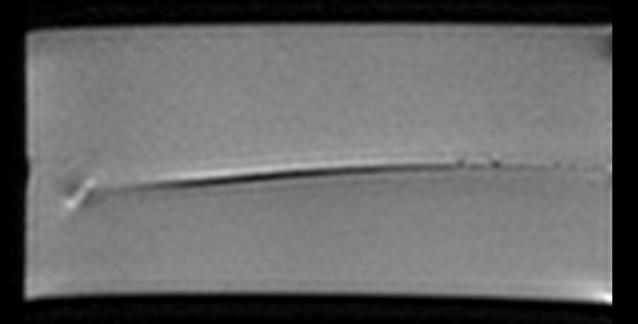
\includegraphics[width=1.0\textwidth]{Fig/chap1/mri_phantom.png}
\caption{MRI scan of a gelatin tissue phantom undergoing needle insertion. The needle enters the phantom at the right of the image. Note the artifact around the needle tip.}
\label{fig:mri_phantom}
\end{figure}


\section{Tissue Phantoms}
Synthetic tissue phantoms are often used during needle insertion studies instead of ex-vivo tissue specimens. These phantoms are designed so their mechanical properties reflect those of human tissue. They offer several benefits over real tissue, especially in the context of benchtop laboratory experiments.
\begin{enumerate}
\item Phantoms made of gelatin or plastic are transparent, so vision-based methods can be used for needle tracking or for validation of other imaging modalities.

\item A needle inserted into a homogeneous tissue phantom will experience constant cutting force throughout insertion.

\item Phantoms can include multiple regions with different mechanical properties separated by membranes.

\item Phantoms have a much longer shelf life than tissue, granting more flexibility to studies.
\end{enumerate}


\begin{figure}[h]

\includegraphics[width=1.0\textwidth]{Fig/placeholder.png}
\caption{Gelatin tissue phantom similar to the ones used in this thesis.}
\label{fig:gelatin_phantom}
\end{figure}

% \section{Medical Image Processing Software}
% \subsection{3D Slicer}
% 3D Slicer is an open-source GUI-centered tool for performing medical image processing and image-guided procedures. It provides a common standard and familiar interface for medical researchers. Algorithms developed by research into medical imaging are frequently released as Slicer modules.

% \subsection{OpenIGTLink}
% OpenIGTLink is a communication standard for image-guided therapy (IGT) that supports sending and receiving images, DICOM data, and 3D homogeneous transforms between devices and programs via TCP/IP. 3D Slicer includes an OpenIGTLink extension to allow communication with imaging devices like MRI and ultrasound and control of robotic surgical tools.



% \section{Thesis Overview}
% \label{sec:Overview}
% \subsection{Needle Model Integration}
% Previous work in needle localization has focused on applying computer vision and image processing algorithms to find the needle tip in camera images and MR data. Particular emphasis has been placed on the calculation of needle positions and orientations for closed-loop control of a robotic insertion system. A useful capability not demonstrated so far would be the use of a mechanical needle model to calculate the expected needle position given the previous needle state and the known inputs at the robot/needle interface, which could be used by the imaging and needle localization systems to improve the imaging rate or measurement accuracy.

% \subsubsection{Needle Model Implementation}
% The kinematic model proposed by \cite{WebsterModel} has already been implemented and extended by various authors, so it would be a reasonable starting point for needle localization augmentation. I have a working Python implementation of this model.

% The addition of torsional dynamics accounting for variable needle depth in the dynamic model shown in \cite{SwensenDynamics} would be useful when working with the thin nitinol needles used to demonstrate small-radius needle steering. The model in \cite{SwensenDynamics} is considerably more technically complex than models in \cite{WebsterModel} or \cite{ReedDynamics}, but I have developed a tentative implementation for an RBE502 Robot Controls project.

% Challenges with needle modeling:

% - Many models assume that the needle isn't rotated during insertion, and that the deflection is effectively only in one direction.

% - Need to represent any conceivable bending configuration

% - Limited measurements to fit FEA mode

% - Can't measure twist within the needle

% \subsection{Improved Needle Localization}

% \subsubsection{Needle Localization via Cross-Section}
% - Use needle model and bot kinematics to estimate tip depth
% - Conduct scan just behind estimated tip position
% - Measure actual needle cross section position
% - Update model to reflect actual needle behavior
% - Reduced dependence on capturing tip in scan plane, less likely to completely lose needle
% - Benefits from small FOV
% - Use FFE sequence to minimize needle shaft artifact 

% \subsubsection{Sizing of Imaging Planes}
% The imaging strategy in \cite{AIMNeedleSteering} used conservative imaging parameters to show that closed-loop control of the imaging planes could keep the needle tip within the imaged volume throughout insertion. A comparatively large slice thickness of 10mm was required to guarantee that the imaging planes would never lose tracking during insertion. Extending this system to make model-based predictions of needle behavior would allow the system to move the imaging planes in anticipation of the motion of the needle tip. While the current approach sizes the thickness of the imaging planes to accommodate any possible tip motion between imaging updates, under a model-based approach the slice thickness would be designed around the error between the modeled and actual motion of the needle tip. Under a well-designed model with physically-representative system parameters, this approach would be more accurate than previous efforts. The measured position of the needle tip could update the state of the dynamic model, which would prevent the model from diverging from the actual behavior of the needle during insertion.

% \subsection{Alternative Imaging Strategies}
% The 2Hz scan rate achieved by \cite{AIMNeedleSteering} represents a baseline and a possible starting point for improvement. The approach used in \cite{AIMNeedleSteering} is to take alternating scans in the coronal and sagittal planes, where the plane of each scan is chosen based on the position of the needle detected in the previous scan in the other plane.  If the position of the needle during insertion is known with some certainty, then a different imaging approach could be used. One option could be to reduce the thickness of the plane, which would improve the visibility of anatomy near the needle but could increase the risk of losing tracking on the needle during insertion.

% Another option could be to use a volumetric scan, which would provide voxel data that would determine the 3D needle tip position. A volumetric approach could be more tolerant of off-axis insertion directions, but it would require a significantly different data processing strategy than the current 2D imaging sequence. It might also be too difficult to successfully implement within the scope of this project.

% In the context of project work, making modifications to the 2D plane method would be more likely to result in a working system, and the volumetric approach could be researched and implemented later in the project once the capabilities and limitations of the MRI machine and its software are more completely understood.

% \subsection{Alternative Scan Plane Orientation}
% The coronal/sagittal plane strategy used in \cite{AIMNeedleSteering} assumes that the needle will always be inserted coaxially with the bore of the MRI machine, and that its direction will not significantly deviate during insertion. Modeling of 6-DOF needle pose, coupled with measurement of needle pitch and yaw, would provide sufficient data to realign the scan planes to keep the planes tangential to the tip of the needle. While this would present added complexity in the form of frequently-updated transforms for the scan planes, it could provide better tip localization results, especially if the scan plane is much thinner than the 10mm baseline from \cite{AIMNeedleSteering}.

% \subsection{Real-Time Control}
% Since real-time needle guidance is the ultimate goal of the project, care should be taken that the chosen implementations do not preclude processing times less than the MRI scan rate. It would also be beneficial to experimental data collection if closed-loop insertion trials could be completed quickly.

% \subsection{Slicer Module}
% Releasing the above functionality as a Slicer extension would facilitate future research and extension by other groups. The robots used in the AIM Lab are generally designed to communicate via OpenIGTLink, which is already built into Slicer.
% - Get more eyes on the research, facilitate transfer to future student

% \subsection{Supporting Simulation Software}
% The capability to conduct tests independent of the availability of MRI equipment and a suitable insertion platform is highly desirable, especially during the evaluation of steering algorithms. Two pieces of software separate from the Slicer module are required. The first is a kinematic simulator of the insertion robot that can conduct a constant-velocity insertion profile while publishing the pose and velocity of the base of the needle. The second is a simulated MRI scanner, which chooses a volumetric scan from a timestamped series to match the current state of the insertion platform and resections a 2D scan using the field of view and scan plane pose provided by the Slicer module. This combination of utilities will be sufficient to 

% \section{Logistics}
% \subsection{Schedule with Coursework}
% In order to meet the requirements of the thesis-based RBE MS, I will need to complete two more credit-hours of coursework in addition to the nine credit-hours of thesis work. I plan to finish my coursework by taking RBE550 Motion Planning in the Spring semester. I would like to divide research credits approximately equally between the semesters, with five in the Fall and four in the Spring.
% \subsection{Lab Work Hours}
% My experience with my directed research project this past Spring improved my understanding of the extent and distribution of work needed to research, implement, test, and document a component in a robotic system. I initially expected to spend about eight hours per week in the lab, split between Tuesdays and Thursdays, with additional hours to be added as needed. During the week of "crunch time" leading up to the paper submission, I spent about 6 hours per day in the lab, plus extra time during the adjacent weekends. I expect that a consistent 20 hours per week would give enough time to complete the project objectives, with extra time available to conduct experiments using the MRI equipment.
% \subsection{Deadlines and Deliverables}
% A key part of the needle tracking project, and one not present in my initial plan submitted in January, was the push for publication in March. The timeline and work items for my thesis research should be built around known similar goals, and should be sufficiently flexible to accommodate emerging opportunities. It would be reasonable to plan to have the foundational research finished by September and the individual software components prototyped by the end of December 2017, which would leave ample time for iteration and additional development through the end of Spring 2018.

% Marek-motivated papers (Hamlyn, haptics, MRI)

% March IROS journal paper and conference submission deadline

% WPI Master's thesis dissertation paper (this document!)

% Slicer modules: MRI simulation module, needle modeling and tracking module

% Python scripts: stereo needle tip localization and pose estimation

% \subsection{Planned Experiments}
% \subsubsection{Full Phantom Scan Series}
% Insert a needle into the phantom and take full volumetric scans at regular depth intervals. This data will form the basis of the Slicer MRI simulator.

% Does resectioning a volumetric scan in an arbitrary plane produce different results in terms of artifacts, noise, etc than taking a new scan in that plane?
% \subsubsection{MR Needle Tracking Verification}
% Demonstrate tracking by following a needle in real-time in an actual MRI environment. Requires communication of desired scan plane to the MRI machine via its API, which depends on the availability of a compatible MRI machine.
% \subsubsection{CV Tracking Verification}
% Might be a good idea to do the same as above with the stereo needle tracking rig.

% \subsection{Work Items}
% \begin{itemize}
%   \item Learn MRI machine software API and system interface.
%   \item Evaluate practical feasibility of proposed goals, especially volumetric imaging and scan plane rotation.
%   \item Adapt existing needle kinematic and dynamic models to be compatible with needle localization software.
%   \item Devise metrics to show improvement of new tracking algorithm compared to prior efforts.
% \end{itemize}

% \section{Methods}
% \subsection{Needle Detection}
% - Need to sample cross-section points in imagery, to capture needles in "slices".

% - Strategy is similar between different imaging modalities.

% - In MRI, needle is inserted normal to the axial plane, so the axial slices contain cross-sections of the needle artifact. Threshold each slice to find dark regions, find contours in 2D, and assume that the centroid of the contour closest to the modeled needle is the coordinate of the needle section. Assumes a simplified model for needle artifacts and a limited range of needle insertion trajectories.

% - Stereo video is used to track the needle in 3D through transparent tissue phantoms. Emulate behavior of MRI by finding coordinate of needle cross section in a specified plane. Assume needle moves nearly horizontally across camera images. Estimate needle tip coordinate from needle model. Take a column of pixels near the tip coordinate, threshold between light and dark pixels, and find the centroid of the dark region closest to the estimated tip coordinate. Assume that this point lies on the needle shaft. Using matching needle points found in each image, triangulate an estimated 3D point using camera intrinsic and extrinsic parameters. The degree of the polynomial curve fit is a variable that can be adjusted.

% - There are two strategies for measuring needle points. We could measure only points close to the tip of the needle. This gives us more updates close to the needle tip, but it assumes that the needle shaft exactly follows the trajectory of the tip, which doesn't hold in soft material. Another option is to resample at different points along the needle shaft. This could present problems in MRI, where each new imaging plane consumes scanning time, but it allows the entire needle model to be updated at once. The frequency of imaging and the spacing between resampling planes are variables.

% \subsection{Needle Insertion Platform}
% - Used a simple PLA needle guide to center the needle on the phantom during MRI data collection. Plastic spacers on the needle shaft allow the needle base pose to be calculated at each insertion step.

% - Used 6-DOF insertion robot during visual needle tracking evaluation. Needle pitch and yaw and translational elements are set before insertion, while needle depth and role are controlled throughout insertion.

% \subsection{Software Architecture}
% - OpenIGTLink to and from robot, can use Slicer to simulate robot comms

% - MRI control via OpenIGTLink. Pick scan planes and field of view.

% - INSERT SYSTEM DIAGRAM FIGURE

% - Module for real-time needle tracking in MRI.

% - Listener registered to volume from MRI, runs segmentation when callback is triggered by update

% - Simple ITK used for segmentation, VTK used for homogeneous transforms

% \subsection{Experimental Setup}
% - MRI data collected for a homogeneous agar gelatin phantom. Needle inserted at regular intervals, full volume collected using XX protocol. Voxel size of 0.4mm x 0.4mm x 0.5mm. Compare estimated tip position from model against manually-labeled tip positions in each volume.

% - Stereo vision localization validates real-time approach and communication with robot. Insert needle into homogeneous plastisol phantom with stiffness XX

% - Use robotic insertion platform detailed in previous paper [cite Marek]

% \section{Results}
% - Note: fill in with actual results

% \subsection{Stereo Needle Tracking}
% - Competing standard would be manually-labeled needle points and tip orientation

% - With live tracking, can show that we actually successfully track the needle to a target

% - Try for simple case (no rotation) and increasingly rigorous cases (thin needle, many curves, significant deflection)

% - Methods to evaluate:

% - linear and polynomial regression for all needle points

% - Piecewise polynomial minimum bending energy model (3rd and 5th degree)

% - Track tip positions vs resample along needle shaft

% - Plots: Example insertion for each with curve overlaid. Error for tip pose.

% \subsection{MRI Needle Tracking}
% - MRI data is limited and very simple: no rotation, deflection in just one direction. Can't do live tracking. Need to show that model accurately finds needle points in each slice and gives a good estimate of the needle tip pose.

% - Plots: Curves overlaid on scans.



% \subsection{Timeline (In Development)}
% \begin{tabular}{| l | l|}
%     \hline
%     Date & Milestone \\ \hline
%     2017 \\ \hline
%     September & Foundational Research Finished; Select Needle Dynamic Model \\ \hline
%     October & Demonstrate Existing MRI Tracking System \\ \hline
%     November & Prototype Key Software Components of New Tracking System \\ \hline
    
%     2018 \\ \hline
%     January & Demonstrate New Needle Tracking and Closed-Loop Scan Plane Control \\ \hline
%     February & Data Collection and Design Iteration \\ \hline
%     Mid/Late-March & Prepare Presentation and Documentation \\ \hline
%     Mid-April & Defense \\ \hline
% \end{tabular}

% \section{Conclusion}
% The extension of current research in needle localization and guidance to include model-based estimation of the needle tip during insertion would be of appropriate scope for a MS thesis project.

% \subsection{Goals}
% - Model needle tip pose throughout insertion into a homogeneous medium using the pose of the needle base and the mechanical properties of the needle.
% - Use this pose to choose a MRI scan plane that captures the actual needle position at or very close to the needle tip.
% - Use this measurement to update the needle model and correct for unmodeled deflection.
% - Bundle this functionality as a Slicer module.
